\chapter{基于FDTD的理论仿真}
\label{cha:simulation}

\section{基于GST的可变超表面光学器件结构研究}
\label{sec:second}

我们决定在如图 ~\ref{fig:metaunit}  \cite{GSTnk} 的结构基础上进行优化,这种结构最明显的优点是可扩展性:当在横向增加GST柱子的个数时,GST相变前后导致的折射率变化可以产生更多的可能的调制状态。然而与此同时,结构单元尺寸的增加会导致能够调节的光波长增加,而将三个纳米柱视为一个结构单元是比较折中的一个选择。
\begin{figure}[H] % use float package if you want it here
  \centering
  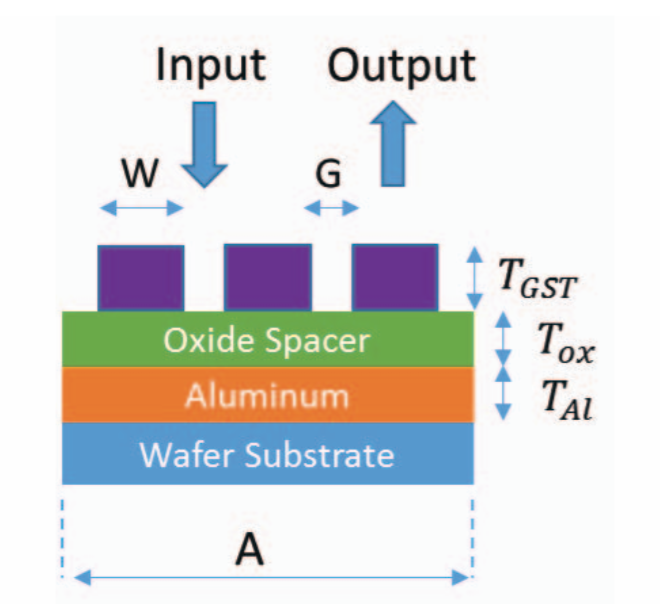
\includegraphics{metaunit.png}
  \caption{可调节纳米柱的结构单元} \cite{GSTnk}
  \label{fig:metaunit}
\end{figure}

在图~\ref{fig:metaunit}所示的结构单元中,每个单元中有三个尺度约为100 nm,间距为47 nm的GST纳米柱。这三个纳米柱排布在50 nm厚的氧化层上,同时加上了铝沉底用来将此结构用作反射器件。根据文献中表明,此结构可以实现在$\left (0,\ 2\pi \right )$范围内的相位调制,但是可调节的相位数目很少。因此,本论文将仿真主要目的集中在增加GST阵列可调节的相位数目。

同时,由于文献 \cite{GSTnk} 中采用的是一维结构,这导致了一个尺度接近$1 \mu m$的结构单元中只有三个纳米柱,而这是一种对空间的浪费。在后续仿真中,我们尝试在一个结构单元中使用$3 \times 3$个GST纳米柱,这样的好处是能够在结构单元尺寸不发生变化的情况下将自由度提升到了原来的平方。

\section{FDTD仿真}
本论文采用FDTD方法对文献所述的功能可调的超表面光学器件单元结构进行仿真与优化。
\subsection{FDTD方法简介}
\label{subsec:fdtd}
FDTD(Finite-Difference Time-Domain),时域有限差分法,核心思想在于把时域麦克斯韦方程转化成差分形式,进而采用数值方法求解。它实现了将计算机不方便处理的旋度方程向差分方程的转化,从而让计算机能够高效地介入电磁场求解的过程中。

以一维麦克斯韦方程为例,在一维场合中,x, y均不影响场量或者介质参数,因此可以表示为
\begin{displaymath}
\frac{\partial E_{x}}{\partial t} = -\frac{1}{\epsilon _{0} \epsilon _{r}} \cdot{} \frac{\partial H_{y}}{\partial z} \qquad \frac{\partial H_{y}}{\partial t} = -\frac{1}{\mu _{0}\mu _{r}} \cdot{} \frac{\partial E_{x}}{\partial z}
\end{displaymath}
使用差分对一阶导数进行近似,我们可以得到
\begin{equation}
\frac{E^{n+1}_{x}(k) - E^{n}_{x}(k)}{\Delta t} = -\frac{1}{\epsilon _0\epsilon _{r}(k)} \cdot{} \frac{H^{n+\frac{1}{2}}_y \left (k+\frac{1}{2} \right) - H^{n+\frac{1}{2}}_y \left (k-\frac{1}{2} \right )}{\Delta z}
\end{equation}
\begin{equation}
\frac{H^{n+\frac{1}{2}}_y \left (k + \frac{1}{2} \right ) - H^{n-\frac{1}{2}}_y \left (k+\frac{1}{2} \right )}{\Delta t} = -\frac{1}{\mu _0\mu _r \left (k+\frac{1}{2} \right )} \cdot{} \frac{E^n_x \left (k+1 \right) - E^n_x \left (k \right )}{\Delta z}
\end{equation}
根据以上两个方程,并使用归一化磁场
\begin{displaymath}
\stackrel{\sim}{H} = \sqrt{\frac{\mu _0}{\epsilon _0}}H
\end{displaymath}

和真空中光速
\begin{displaymath}
c = \frac{1}{\sqrt{\mu _0 \epsilon _0}}
\end{displaymath}

代入,可以得到基于FDTD的迭代公式:

\begin{equation}
\stackrel{\sim}{H}^{n+\frac{1}{2}}_{y} \left (k + \frac{1}{2} \right ) = \stackrel{\sim}{H}^{n - \frac{1}{2}}_y \left (k + \frac{1}{2} \right ) - \frac{c\Delta t}{\mu _r\left (k + \frac{1}{2} \right ) \Delta z} \cdot{} \left ( E^n_x (k + 1) - E^n_x (k) \right )
\end{equation}

\begin{equation}
E^{n + 1}_x \left (k \right ) = E^n_x \left ( k \right ) - \frac {c \Delta t}{\epsilon _r \left (k \right ) \Delta z} \cdot{} \left ( \stackrel{\sim}{H}^{n + \frac{1}{2}}_y \left (k + \frac{1}{2} \right ) - \stackrel{\sim}{H}^{n + \frac{1}{2}}_y \left (k - \frac{1}{2} \right ) \right )
\end{equation}

由于结构参考的文献中采用的是一维结构,而超表面本身蕴含的结构不超过二维;因此对于三维FDTD方程的推导是不必要的。

基于以上原理,我们采用FDTD方法对超表面结构进行仿真。有关仿真的具体过程,在此不加以赘述,只进行一些必要的对结果的讨论。

\subsection{一维情形}
\label{subsec:onedim}
本论文首先实现了对文献所述结构的仿真优化。其中需要的GST材料在可见光-近红外波段的复折射率参数由文献 \cite{GSTnk} 中的曲线粗略得到。有关GST材料在晶态/非晶态的详细折射率如图 ~\ref{fig:nkGST} 所示。
\begin{figure}[H] % use float package if you want it here
  \centering
  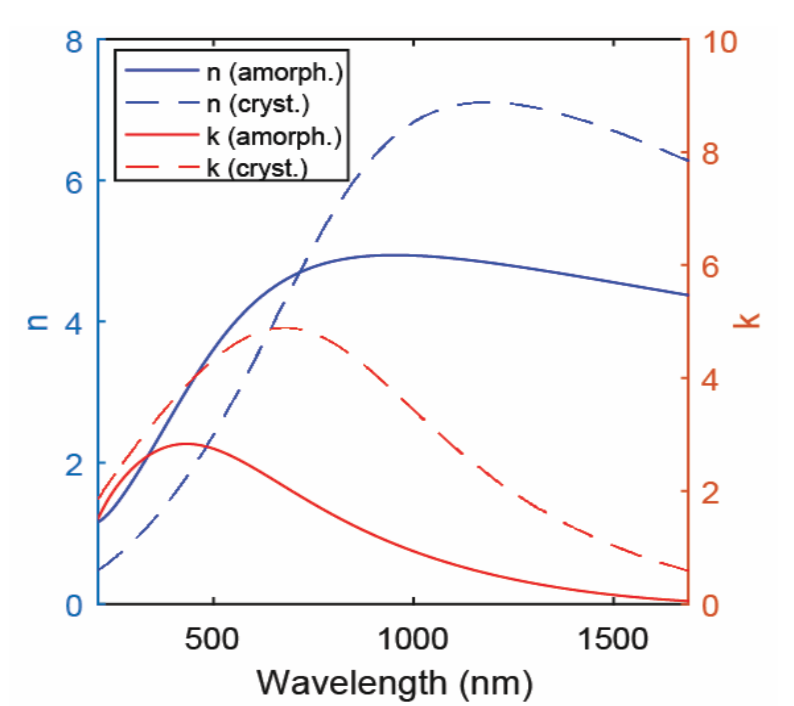
\includegraphics[width=0.5\textwidth]{GSTnk1.png} \cite{GSTnk}
  \caption{GST材料在可见光以及附近的折射率和消光系数}
  \label{fig:nkGST}
\end{figure}

本论文首先进行了对文献中所示结构的验证。一维情况下的结构如图 ~\ref{fig:dstructure} 所示:
\begin{figure}[H] % use float package if you want it here
  \centering
  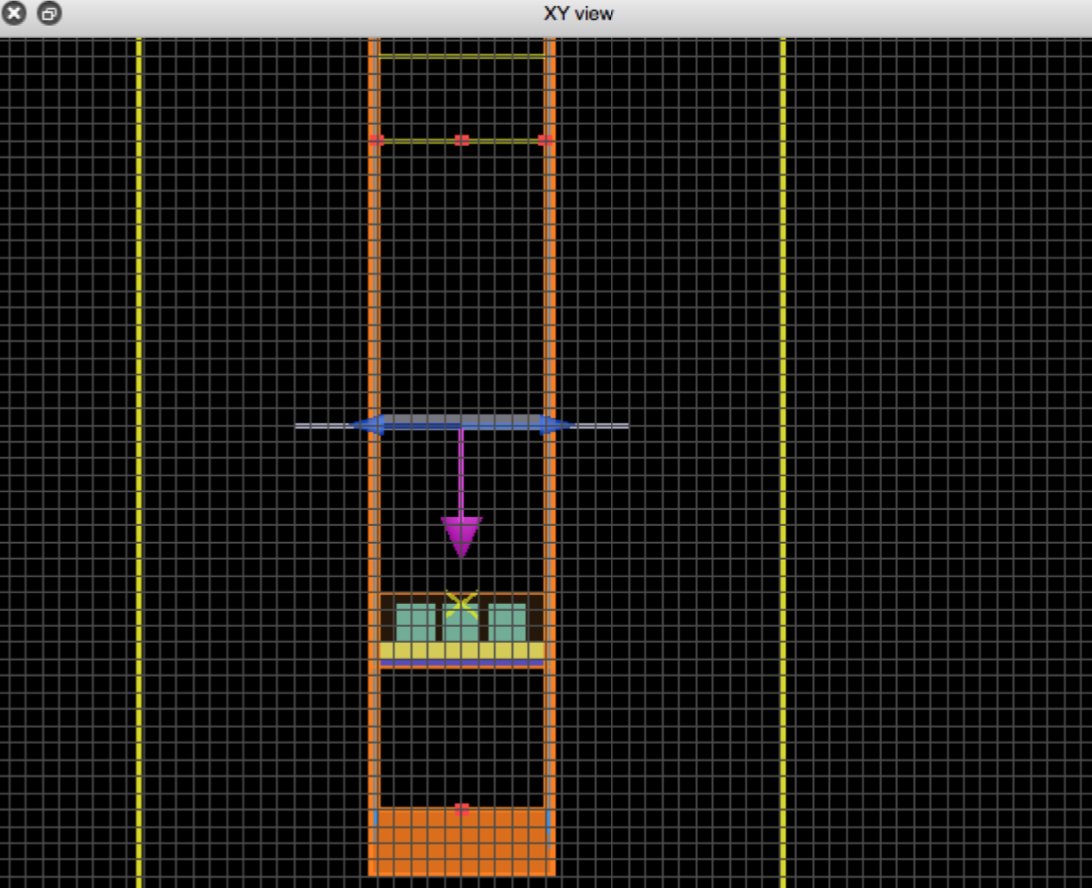
\includegraphics[width = 0.6\textwidth]{1dstructure.png}
  \caption{一维纳米柱结构示意图}
  \label{fig:dstructure}
\end{figure}

其中,三个矩形表示了GST形成的纳米柱。通过预先调入非晶化和晶化状态下的GST材料的$\left (n,k \right )$,我们可以通过设定与更改这三个矩形的材料属性来模拟晶化和非晶化的过程。如果我们用a表示非晶态的GST,而用c来表示晶态的GST材料,那么考虑到对称性,这三个纳米柱组成的结构单元共有$\left (aaa \quad aac \quad acc \quad aca \quad ccc \quad cac \right )$六种状态。由于我们期待着的是一个具有可重复性的结构单元,因此我们将边界条件设置为周期性边界条件来进行仿真。
我们可以得到以下相位曲线:
\begin{figure}[H] % use float package if you want it here
  \centering
  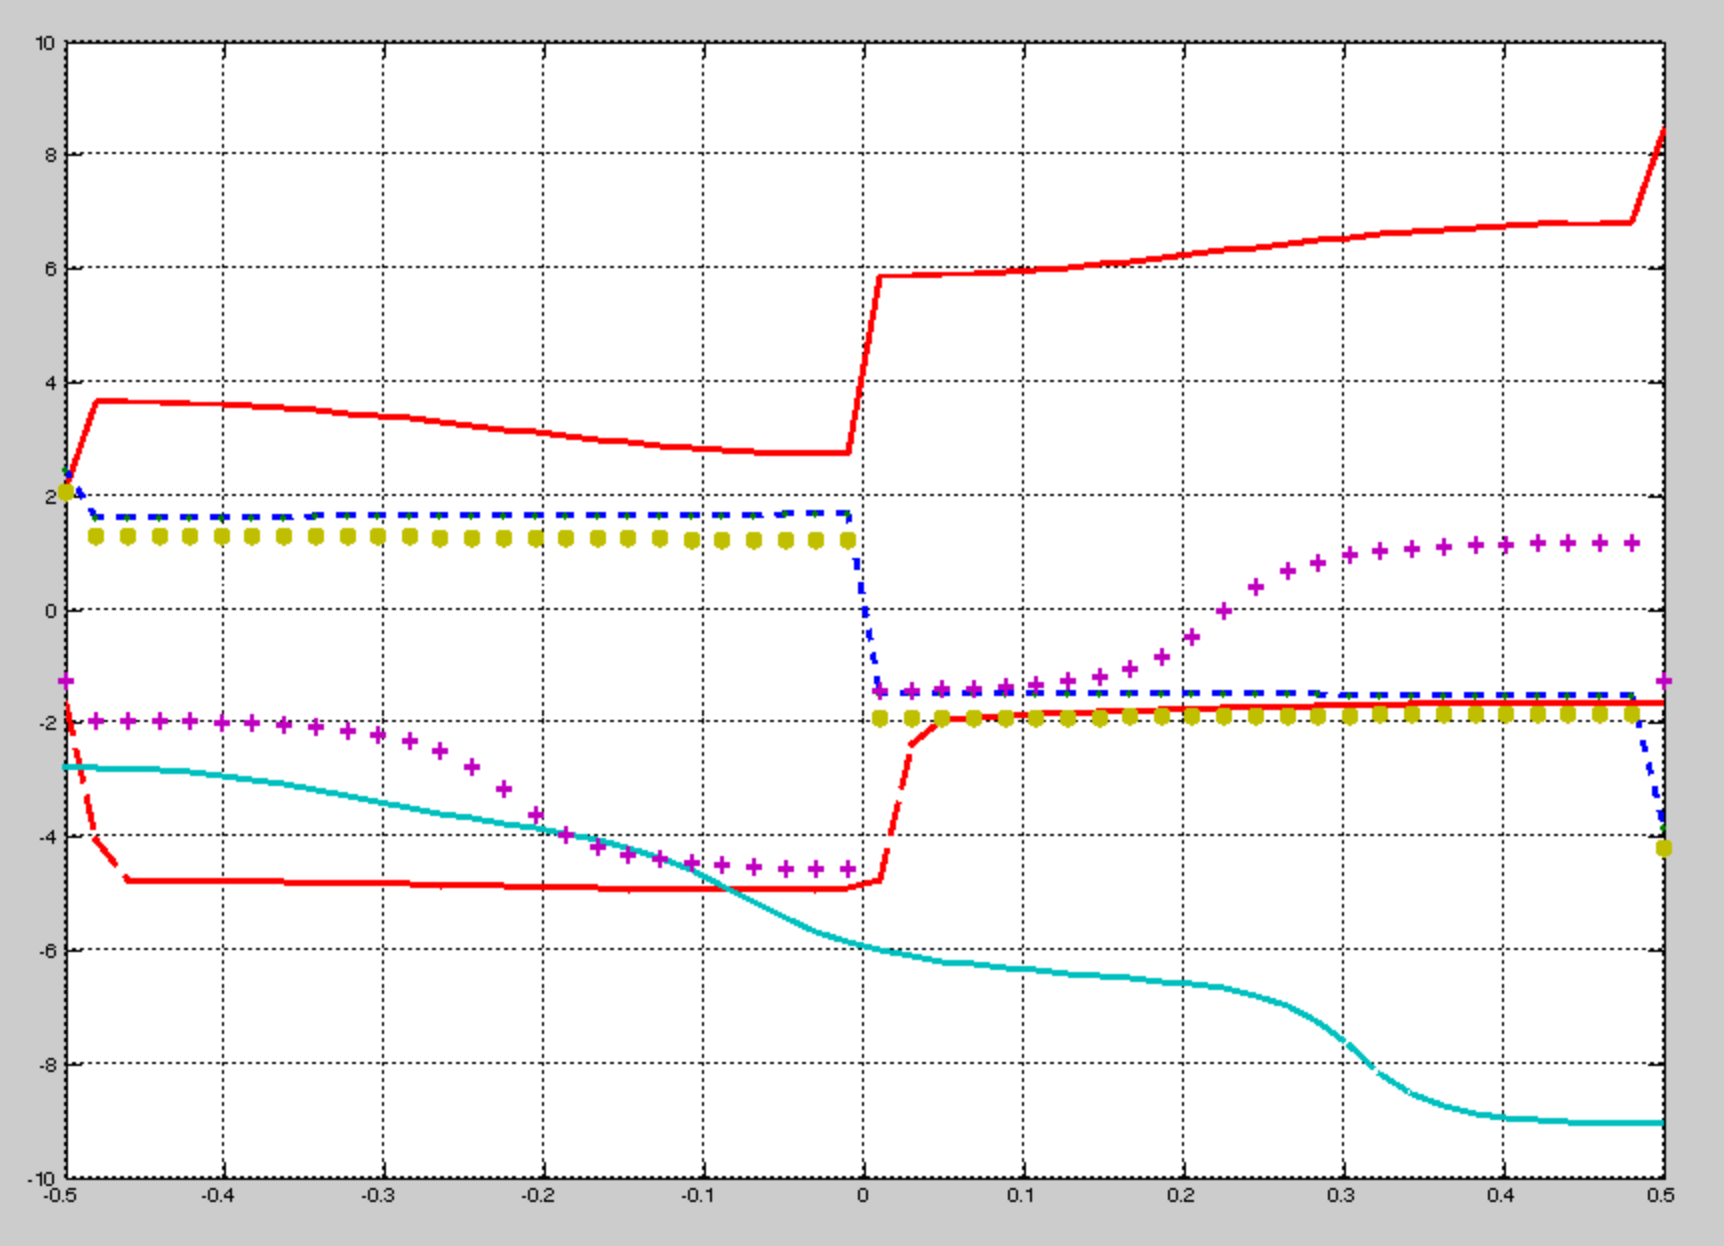
\includegraphics[width = 0.5\textwidth]{1dphase.png}
  \caption{对一维GST纳米柱组合形成的相位分布示意图}
  \label{fig:1dphase}
\end{figure}
零点处的相位随着GST材料晶化状态的仿真结果与文献所述 \cite{metaGST} 十分接近,说明本论文所述的仿真过程和结果是可靠的。但是,在一维情形下,零点附近的相位变化十分剧烈,而零点的相位变化又是我们希望严格受控的,因此在零点附近如此剧烈的相位变化应当在我们后续的结构设计中得到控制。

\subsection{二维情形}
\label{subsec:twodim}
对二维情形的仿真所用到的GST材料的复折射率,同样是基于参考文献 \cite{GSTnk} 中的曲线得到。

二维结构下的结构如图 ~\ref{fig:twodim} 所示,在一维的基础上增加了y方向的结构;除此之外,将纳米柱的形态确定为全等的圆柱体。如下图所示,此超表面的结构单元尺寸约为$1\ \mu m$,仿真所用的光源和检查的平面与反射衬底的底面距离分别为500 nm, 510 nm。
\begin{figure}[H] % use float package if you want it here
  \centering
  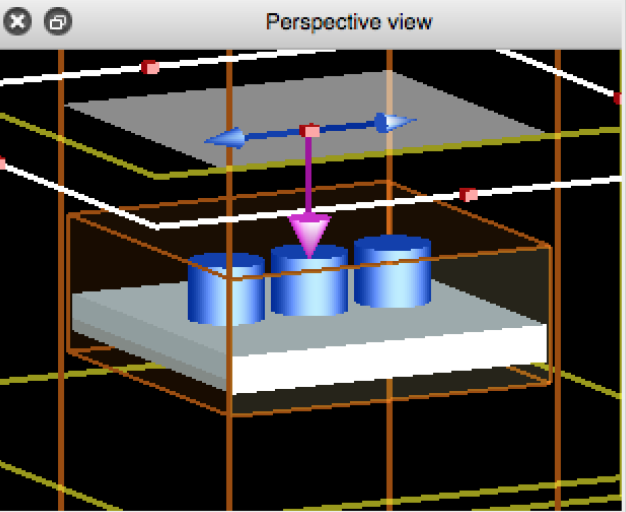
\includegraphics[width = 0.5\textwidth]{twodstructure.png}
  \caption{二维纳米柱结构示意图}
  \label{fig:twodim}
\end{figure}

由于在同一个结构单元内,每个GST纳米柱有晶化和非晶化两种状态,因此在不考虑对称性的情况下一个单独的二维结构单元能够实现$2^9=512$种不同的相位调控。即便考虑对称性,也有86种不用的调节情况(此处的计算用到了P\'olya计数法),远远多于一维情形的六种。为了实现超表面所需的相位调节能力,我们所诉求的是找到尽可能充满$\left (0,\ 2\pi \right )$区间点若干个点。换言之,我们设通过各个GST纳米柱的晶化状态调节能够实现的相位变化集合为A,那么对于任意的$x \in \left (0,\ 2\pi \right )$,均$\exists a \in \mathrm{A}\textrm{和}\delta > 0,\ s.t.\ x \in \left (a - \delta,\ a + \delta \right )$,我们的期望是$\delta$尽可能小。根据经验而言,当$\delta < \pi / 8$时,可以认为基本实现了可控的超表面。

由于二维情况下的可能的晶化种类过多,在此就不一一列举,仅用86种不同的GST纳米柱晶化状态中相位差异较大的两种来说明用GST制作的超表面光学器件具有调节能力:
\begin{figure}[h]
\begin{minipage}{0.3\textwidth}
  \centering
  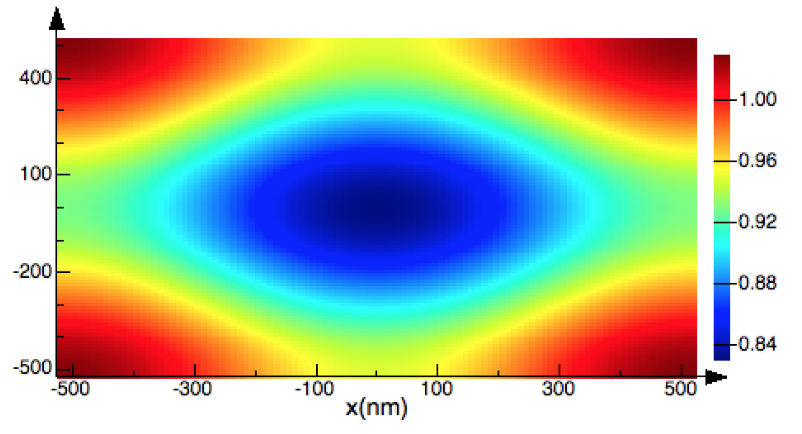
\includegraphics[height = 2.5cm]{tworeflect.png}
  \caption{二维GST纳米柱下的反射强度示意图}
  \label{fig:parallel1}
\end{minipage}\hfill
\begin{minipage}{0.3\textwidth}
  \centering
  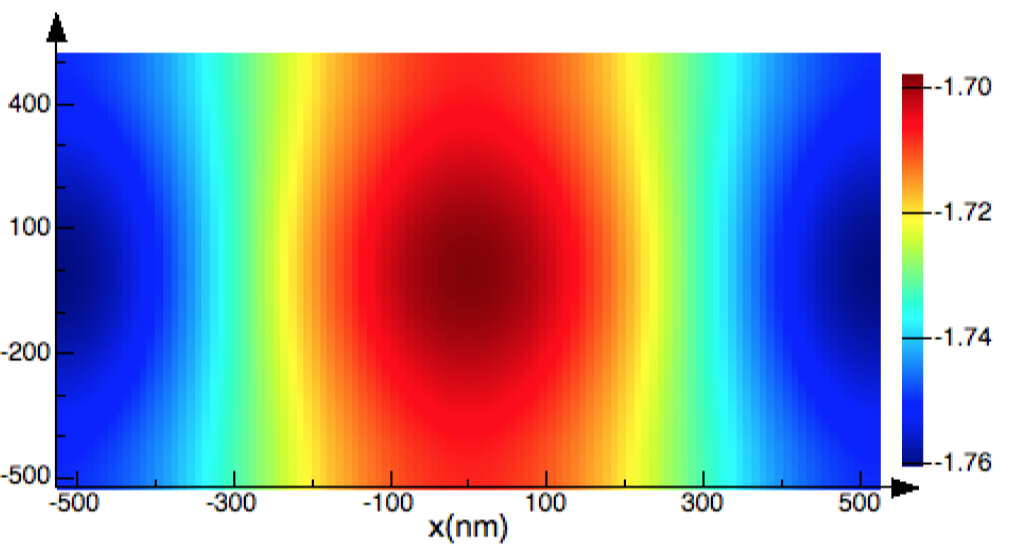
\includegraphics[height = 2.5cm]{twophase1.png}
  \caption{某一个情况下的相位分布}
  \label{fig:parallel2}
\end{minipage}\hfill
\begin{minipage}{0.3\textwidth}
  \centering
  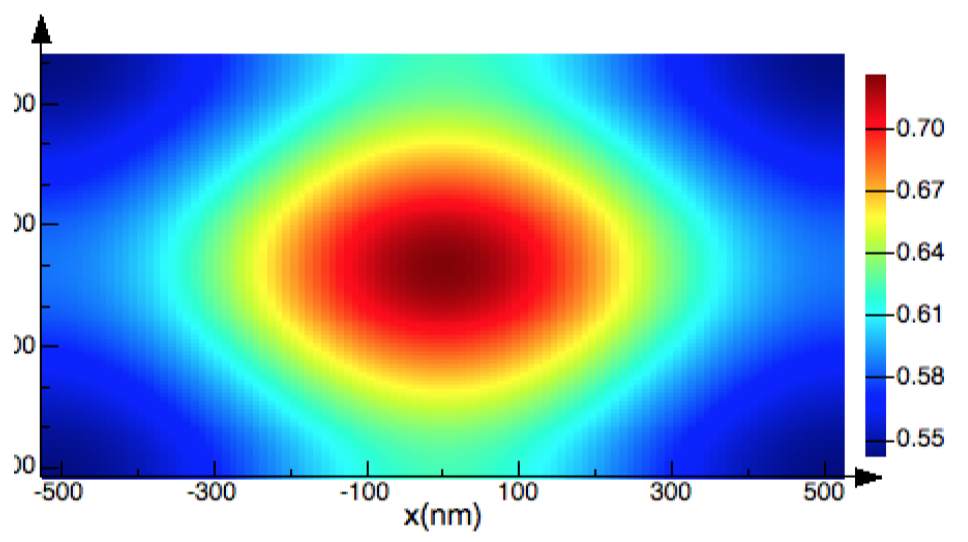
\includegraphics[height = 2.5cm]{twophase2.png}
  \caption{另一个情况下的相位分布}
  \label{fig:parallel2}
\end{minipage}
\end{figure}

从上图中我们可以看出以下几点:
\begin{itemize}
  \item[-] 对于$\lambda \approx 1\ \mu m$的入射光,GST材料的吸收很弱。这说明采用GST制作的超表面光学器件具有损耗小、效率高的特点;
  \item[-] 某个结构单元中各个纳米柱的晶化状态改变前后,在零点处的相位能够有较大的变化;
  \item[-] 无论如何调节某个结构单元中不同纳米柱的晶化状态,零点附近的相位变化是相对平缓的,这是一个明显比一维结构优秀的特点。
\end{itemize}

综上所述,二维结构的调控能力较之一维结构没有本质的提升,但是二维排布的GST纳米柱一维结构所无法比拟的相位稳定性,这使得计算容错性得到提升。

\section{本章小结}
\label{sec:simsumup}
在一维、二维仿真图中,我们可以看到,当把文献所述的GST复折射率采用FDTD仿真时,可以通过GST晶化状态的改变来实现一个能够调控的超表面结构。其中,当GST纳米柱呈一维排布时,零点附近的相位变化跳动比较剧烈;对于二维排布的GST纳米柱,相位平滑程度会好得多。